\chapter{Backend and Data Exposure}

\section{Introduction}
\label{sec:backend-intro}
\begin{sloppypar}
Chapter 1's technology table already gave FastAPI its one-line role in the stack -- ``exposing articles, search, and GenAI endpoints to the frontend'' (Table~\ref{tab:tech-stack}) -- and every chapter since has read a slice of what sits behind one such endpoint without ever stepping back to look at the API as a single surface. Chapter 4 traced the pgvector query behind \texttt{GET /search/}'s primary path (Section~\ref{sec:pgvector}); Chapter 6 opened \texttt{api/\allowbreak routes/\allowbreak genai.py} and \texttt{api/\allowbreak routes/\allowbreak search.py} to describe the LLM calls each endpoint makes (Sections~\ref{sec:genai-summaries}, \ref{sec:ai-search}, \ref{sec:chat-assistant}); and Chapter 7 named \texttt{POST /pipeline/trigger} and \texttt{POST /pipeline/cluster} as the two HTTP entry points into the orchestration layer (Section~\ref{sec:flow-design}). This chapter reads the remaining, connective layer none of those chapters covered: \texttt{api/\allowbreak main.py}, the single file that creates the FastAPI application, configures CORS, and mounts five router modules, one per domain; \texttt{api/\allowbreak routes/\allowbreak articles.py}, the read side of the \texttt{articles} table that every dashboard view in the frontend depends on and that no earlier chapter has opened at all; \texttt{api/\allowbreak routes/\allowbreak img.py}, the same-origin image proxy behind every article thumbnail; and \texttt{etl/\allowbreak load.py}'s \texttt{get\_connection}, the one function every route handler in the codebase calls to reach PostgreSQL. Together they are the whole of what a client of News Insight -- the React dashboard, or anyone reading \texttt{/docs} directly -- actually sees of the backend.
\end{sloppypar}

\section{Backend technology choice}
\label{sec:backend-choice}
\begin{sloppypar}
\texttt{requirements.txt} lists \texttt{fastapi} and \texttt{uvicorn} together under an \texttt{\# API} heading, with no version pin on either -- unlike Prefect's own explicit \texttt{prefect>=3.0.0} (Chapter 7) -- and \texttt{api/\allowbreak Dockerfile}'s final line, \texttt{CMD ["uvicorn", "api.main:app", "--host", "0.0.0.0", "--port", "8000"]}, is what actually serves the application: FastAPI defines the routes, uvicorn is the ASGI server process that runs them. The choice sits on the same simplicity/capability trade-off this report has already named twice -- \texttt{requests}+BeautifulSoup over browser automation in Chapter 3, Prefect over Airflow in Chapter 7 -- weighed here against Flask and Django, the field's other well-known Python web frameworks. Flask is a comparably small ASGI/WSGI surface, but leaves request validation and API documentation to third-party extensions; Django bundles an ORM and an admin site as first-class citizens, which would sit oddly on top of a data layer this report has already shown, and will show again in Section~\ref{sec:data-access}, is deliberately unmanaged, hand-written SQL rather than mapped model classes. FastAPI's own value proposition lines up with what the codebase actually uses it for: Pydantic models double as request-body validation with no extra code, exactly what \texttt{genai.py}'s \texttt{ChatBody} does for \texttt{POST /genai/chat}'s single \texttt{q} field (Section~\ref{sec:chat-assistant}); route signatures typed with plain Python types (\texttt{article\_id: int}, \texttt{limit: int = Query(20, le=100)}) double as query-parameter parsing and bounds-checking; and the framework introspects those same signatures to generate a full OpenAPI schema and an interactive Swagger UI at \texttt{/docs} with no separate documentation step at all (Figure~\ref{fig:screen-apidocs}). One more feature is native to FastAPI rather than layered on top of a generic WSGI app: \texttt{BackgroundTasks.\allowbreak add\_task}, the exact mechanism Chapter 7 already named as how \texttt{POST /pipeline/trigger} and \texttt{POST /pipeline/cluster} fire a long-running job without blocking the HTTP response (Section~\ref{sec:flow-design}) -- a feature the orchestration chapter depends on that a Flask app would need an added task queue to reproduce.
\end{sloppypar}

\section{API structure}
\label{sec:api-structure}
\begin{sloppypar}
\texttt{api/\allowbreak main.py} is short and does exactly three things. First, it instantiates the application: \texttt{app = FastAPI(title="News MLOps API", description="API for Tunisian news scraping, clustering and sentiment analysis", version="1.0.0")} -- the \texttt{title} and \texttt{description} are what render at the top of the Swagger page in Figure~\ref{fig:screen-apidocs}, and \texttt{version} is a plain string the codebase never reads back anywhere else. Second, it adds \texttt{CORSMiddleware} (Listing~8.1) with an explicit, three-origin allowlist -- \texttt{http://localhost:5173} and \texttt{http://127.0.0.1:5173} (the Vite dev server) and \texttt{http://localhost:8000} (Swagger UI's own self-calls) -- \texttt{allow\_credentials=True}, and both methods and headers left wide open with \texttt{"*"}. Third, it mounts five router modules, one per domain, each contributed by its own file under \texttt{api/\allowbreak routes/}: \texttt{app.include\_router(pipeline.router, prefix="/pipeline", tags=["pipeline"])}, and the same call repeated for \texttt{articles} (\texttt{/articles}), \texttt{search} (\texttt{/search}), \texttt{genai} (\texttt{/genai}), and \texttt{img} (\texttt{/img}) -- the \texttt{tags} argument is what groups endpoints into the five labelled sections visible in Figure~\ref{fig:screen-apidocs}'s Swagger page. A sixth route, \texttt{GET /health}, is defined directly on \texttt{app} rather than through any router, returning a bare \texttt{\{"status": "ok"\}}; no \texttt{healthcheck} block for the \texttt{api} service exists in \texttt{docker-compose.yml} the way Chapter 7 described for \texttt{postgres} and \texttt{prefect} (Section~\ref{sec:monitoring}), so this endpoint is reachable but currently unused by the containerized stack's own liveness checks.
\end{sloppypar}

\begin{verbatim}
app.add_middleware(
    CORSMiddleware,
    allow_origins=[
        "http://localhost:5173",   # Vite dev (direct access / health checks)
        "http://127.0.0.1:5173",
        "http://localhost:8000",   # Swagger UI self-calls
    ],
    allow_credentials=True,
    allow_methods=["*"],
    allow_headers=["*"],
)
\end{verbatim}
\begin{center}
\textit{Listing~8.1: the CORS configuration (\texttt{api/main.py}) -- a small, explicit allowlist rather than a wildcard origin.}
\end{center}

\begin{sloppypar}
That allowlist is narrower than it might first appear necessary, because the dashboard's normal traffic never actually needs it. \texttt{frontend/\allowbreak src/\allowbreak api/\allowbreak client.js} builds its \texttt{axios} client with \texttt{baseURL: '/api'}, a same-origin, relative path in both environments the project ships: in development, \texttt{vite.config.js} proxies every \texttt{/api/*} request server-side to \texttt{http://localhost:8000}, stripping the \texttt{/api} prefix before forwarding it; in the Docker Compose stack, \texttt{frontend/\allowbreak nginx.conf} does the equivalent job, proxying \texttt{location /api/} to \texttt{http://api:8000/} over the compose network with a comment that states the consequence plainly -- ``no CORS, no hardcoded localhost.'' Because the browser only ever calls its own origin in both cases, the CORS middleware is not what makes the dashboard work; it is a narrower allowance for exactly the two cases its own comments name -- a request made directly against \texttt{localhost:8000} rather than through either proxy (manual debugging, a health check), and Swagger UI's ``Try it out'' self-calls from the \texttt{/docs} page it is itself served from.
\end{sloppypar}

\section{Endpoints}
\label{sec:endpoints}
\begin{sloppypar}
Table~\ref{tab:endpoints} lists every route the five routers and \texttt{app} itself expose, with the prefix each router is mounted under already folded into the path. Two small conventions are worth flagging because they affect the exact URL a client must call: \texttt{articles.router} and \texttt{search.router} both declare their list-style endpoint at path \texttt{"/"}, so the full route carries a trailing slash (\texttt{/articles/}, \texttt{/search/}) -- exactly what \texttt{frontend/\allowbreak src/\allowbreak api/\allowbreak client.js}'s call sites use (\texttt{client.get('/articles/', \ldots)}, \texttt{client.get('/search/', \ldots)}); \texttt{img.router}, by contrast, declares its only endpoint at path \texttt{""}, so the mounted route is \texttt{/img} with no trailing slash at all, again matching the one place the frontend builds that URL directly, \texttt{frontend/\allowbreak src/\allowbreak utils/\allowbreak image.js}'s \texttt{`/api/img?url=\${encodeURIComponent(url)}`}. Inside \texttt{articles.py}, ordering also matters: \texttt{get\_article}'s catch-all \texttt{@router.get("/\{article\_id\}")} is declared last in the file, after the four fixed-path endpoints (\texttt{/stats}, \texttt{/topics}, \texttt{/timeline}, \texttt{/regions}) -- FastAPI matches routes in registration order, so a request for \texttt{/articles/stats} resolves to \texttt{get\_stats} rather than being swallowed by the parameterized route beneath it.
\end{sloppypar}

\begin{table}[H]
\centering
\begin{tabular}{|p{1.7cm}|p{4.6cm}|p{7.6cm}|}
\hline
\textbf{Method} & \textbf{Path} & \textbf{Purpose} \\
\hline
GET & \texttt{/health} & Bare liveness probe (\texttt{\{"status": "ok"\}}); not wired into any \texttt{docker-compose.yml} healthcheck. \\
\hline
POST & \texttt{/pipeline/\allowbreak trigger} & Runs the scrape/transform/load pipeline as a FastAPI background task (Chapter 7, Section~\ref{sec:flow-design}). \\
\hline
POST & \texttt{/pipeline/\allowbreak cluster} & Runs BERTopic clustering as a background task (Chapter 7, Section~\ref{sec:flow-design}). \\
\hline
GET & \texttt{/articles/} & Lists articles; filterable by \texttt{source}, \texttt{sentiment}, \texttt{topic\_id}, \texttt{region}, paginated with \texttt{limit}/\texttt{offset}. \\
\hline
GET & \texttt{/articles/\allowbreak stats} & Total article count plus positive/neutral/negative sentiment breakdown. \\
\hline
GET & \texttt{/articles/\allowbreak topics} & Topic distribution (\texttt{topic\_id}, \texttt{topic\_label}, article count), ordered by count. \\
\hline
GET & \texttt{/articles/\allowbreak timeline} & Daily sentiment counts over the last \texttt{days} days (default 30). \\
\hline
GET & \texttt{/articles/\allowbreak regions} & Per-governorate article count and dominant sentiment for the map dashboard. \\
\hline
GET & \texttt{/articles/\allowbreak\{article\_id\}} & Single article by id, including full \texttt{content}. \\
\hline
GET & \texttt{/search/} & AI-assisted semantic search over articles (Chapters 4 and 6). \\
\hline
GET & \texttt{/genai/\allowbreak summary/\allowbreak\{article\_id\}} & Cached or on-demand LLM article summary (Chapter 6, Section~\ref{sec:genai-summaries}). \\
\hline
POST & \texttt{/genai/\allowbreak chat} & ``Ask the news'' retrieval-augmented chat assistant (Chapter 6, Section~\ref{sec:chat-assistant}). \\
\hline
GET & \texttt{/img} & Same-origin, SSRF-guarded proxy for a remote article image. \\
\hline
\end{tabular}
\caption{Every HTTP endpoint exposed by the News Insight API, with each router's mount prefix already folded into the path.}
\label{tab:endpoints}
\end{table}

\begin{sloppypar}
\texttt{api/\allowbreak routes/\allowbreak img.py}, named in the table's last row, has not been opened by any earlier chapter. Its own module docstring states the problem it exists to solve: some sources, lapresse.tn among them, serve a ``forbidden'' placeholder image to a cross-site browser request because their WAF keys off the \texttt{Sec-Fetch-Site}/\texttt{Referer} headers a direct \texttt{<img src="https://lapresse.tn/...">} tag sends. \texttt{proxy\_image(url)} fetches the real image server-side instead, with a same-site \texttt{Referer} and none of the cross-site fetch metadata a browser would add, and returns the bytes through the API's own origin -- exactly the URL \texttt{frontend/\allowbreak src/\allowbreak utils/\allowbreak image.js} builds for every article thumbnail. Because the endpoint accepts an arbitrary \texttt{url} query parameter and fetches whatever it points to, it is guarded against server-side request forgery before any request leaves the container: \texttt{parsed.scheme} must be \texttt{http} or \texttt{https}, and \texttt{\_is\_public\_host} resolves the hostname and rejects it if any resolved address is private, loopback, link-local, reserved, multicast, or unspecified -- blocking a URL like \texttt{http://169.254.169.254/} or \texttt{http://localhost:5432/} from ever being fetched on the server's behalf. A successful fetch is further constrained: the response's \texttt{Content-Type} must start with \texttt{image/} or the endpoint returns \texttt{415}, and the body is streamed in \texttt{64\,KB} chunks with an \texttt{8\,MB} running total, aborting with \texttt{413} the moment that cap is crossed rather than buffering an arbitrarily large response in memory first. The successful response itself carries \texttt{Cache-Control: public, max-age=86400}, so a browser (or an intermediate cache) only re-fetches a given proxied image once a day.
\end{sloppypar}

\begin{figure}[H]
\centering
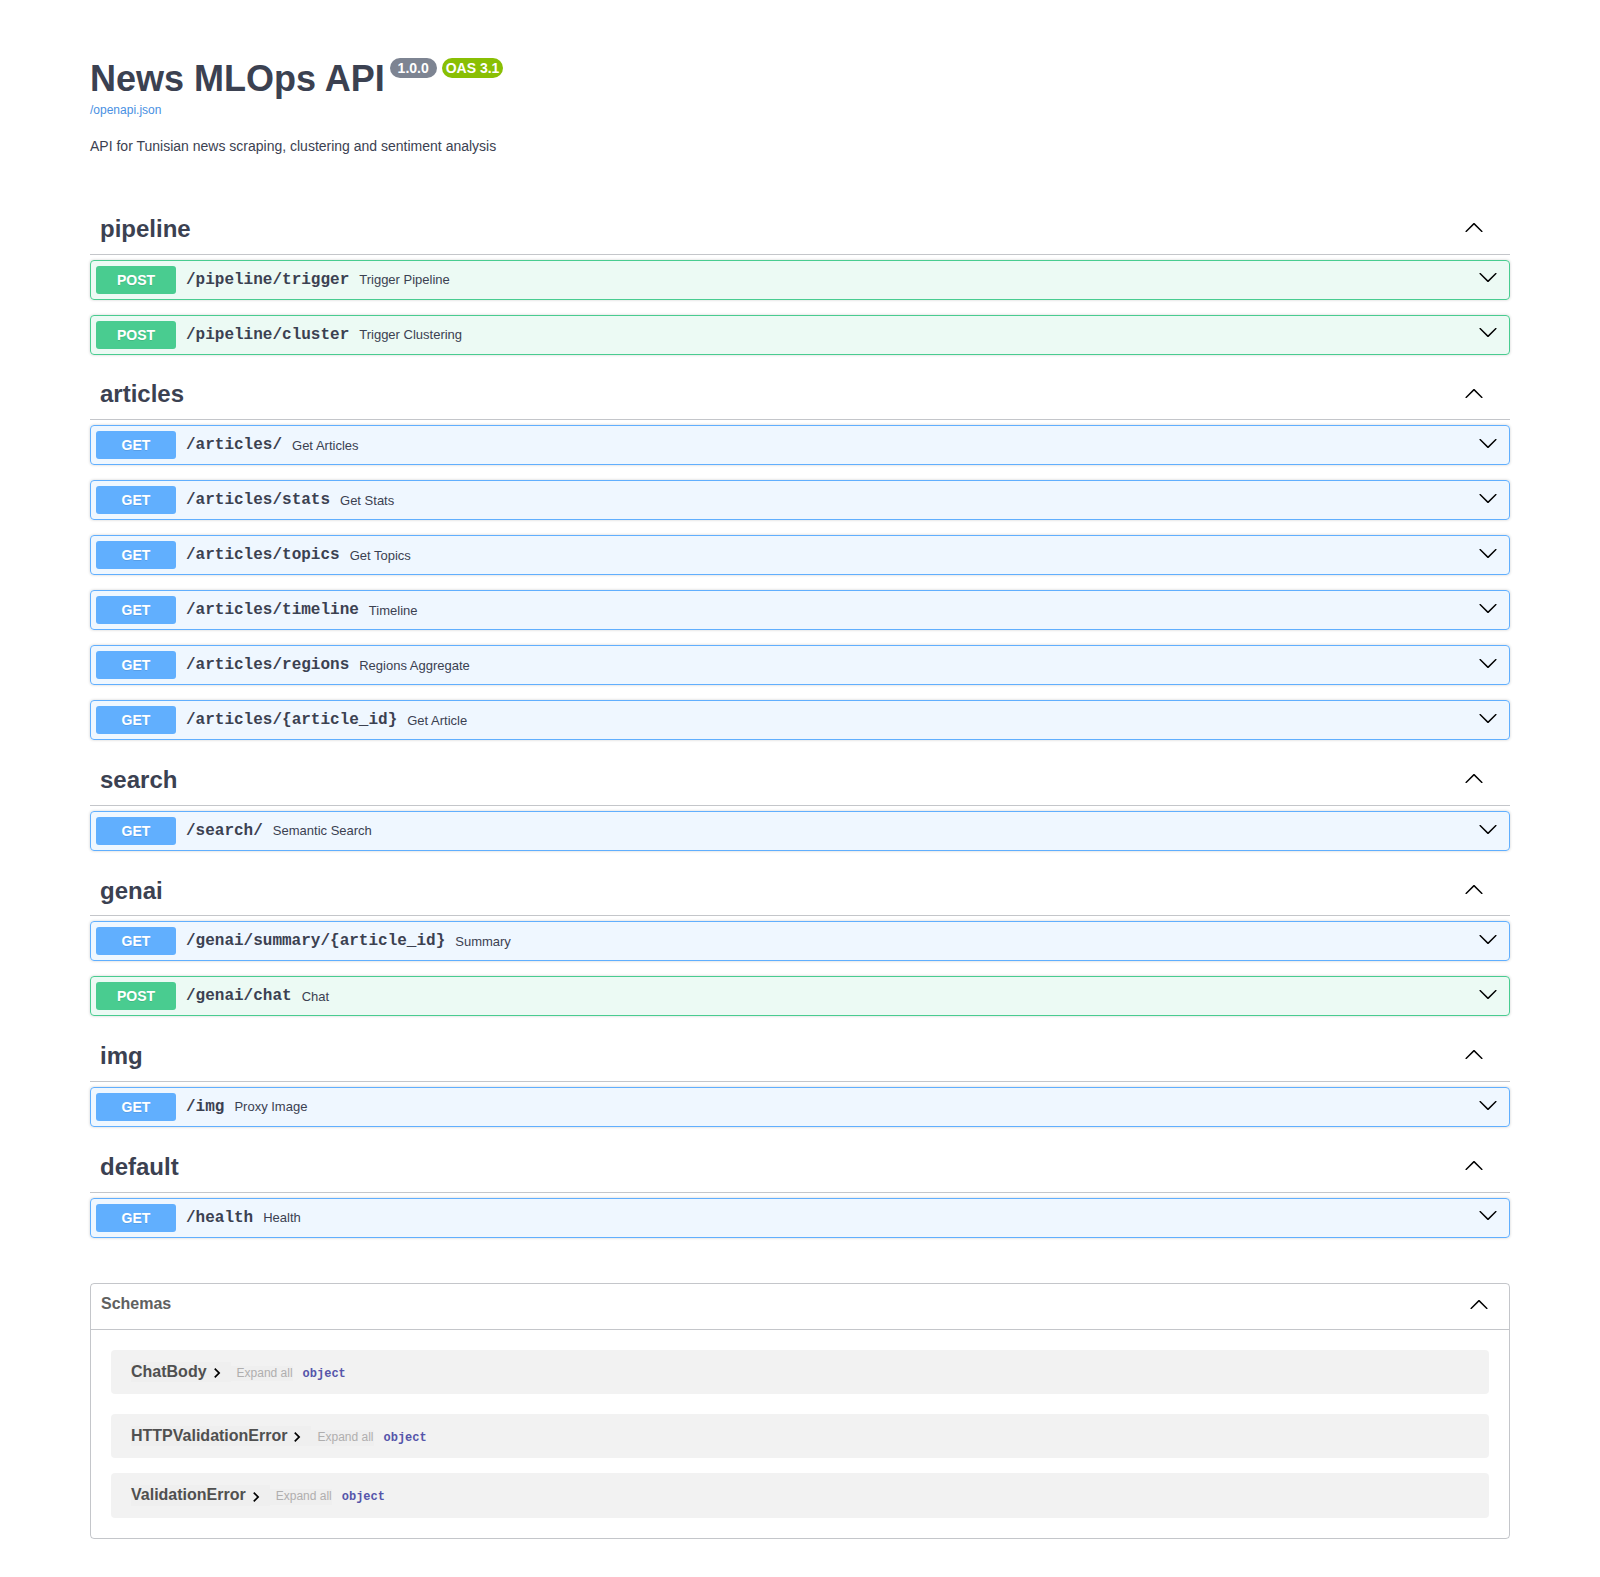
\includegraphics[width=0.9\columnwidth]{img/screen-apidocs.png}
\caption{FastAPI interactive API documentation (Swagger UI) listing the platform's endpoints.}
\label{fig:screen-apidocs}
\end{figure}

\section{Data access patterns}
\label{sec:data-access}
\begin{sloppypar}
\texttt{requirements.txt} lists \texttt{sqlalchemy} under its \texttt{\# Database} heading alongside \texttt{psycopg2-binary} and \texttt{pgvector} -- but no file in the codebase ever imports it. Every route handler across all five routers reaches PostgreSQL the same way Chapter 2 already named for the ETL layer: \texttt{etl/\allowbreak load.py}'s \texttt{get\_connection()}, a single function that opens a fresh \texttt{psycopg2.connect(...)} using \texttt{POSTGRES\_HOST}/\texttt{POSTGRES\_PORT}/\texttt{POSTGRES\_DB}/\texttt{POSTGRES\_USER}/\texttt{POSTGRES\_PASSWORD} read from the environment. There is no model layer between a route handler and the database at all: no declarative table classes, no session object, no query builder -- each handler writes its own SQL string directly, with user-supplied values passed as \texttt{\%s} placeholders that psycopg2 substitutes safely rather than ever being interpolated into the query text. \texttt{get\_articles} (\texttt{articles.py}) is the clearest illustration of what that looks like in practice: it builds its \texttt{WHERE} clause by appending fixed \texttt{"column = \%s"} fragments from a whitelist of four known filters -- \texttt{source}, \texttt{sentiment}, \texttt{topic\_id}, \texttt{region} -- only for whichever ones the caller actually supplied, so the assembled SQL text always comes from the route's own code, never from a client-controlled string, while the corresponding \emph{values} still travel through parameterized placeholders. The \texttt{region} filter carries one special case on top: \texttt{region} values of \texttt{"national"}, \texttt{"null"}, or an empty string are translated to a bare \texttt{"region IS NULL"} clause instead of a parameterized equality check, matching the \texttt{NULL}-as-``National / non-localisé''-bucket convention Chapter 5 already described for articles the region tagger could not place (Section~\ref{sec:enrichment}).
\end{sloppypar}

\begin{sloppypar}
Connection lifecycle is handled with one deliberate exception rather than uniformly. Every handler in \texttt{articles.py} and \texttt{search.py}, and \texttt{genai.py}'s \texttt{chat}, follow the same shape: open a connection, run one or more queries, call \texttt{cur.close()} and \texttt{conn.close()} explicitly at the end of the function body, with no \texttt{try}/\texttt{finally} guarding those closing calls -- so an exception raised by a query itself would skip past them and leave the connection unclosed. \texttt{genai.py}'s \texttt{summary} is the one handler that does not follow that shape, and its current form is the direct result of two commits: \textit{fix(api): always close DB connection in summary endpoint + guard null content} wrapped the handler's body in \texttt{try}/\texttt{finally} so the connection closes on every exit path, including the \texttt{404} raised for a missing article; \textit{fix(api): don't hold DB connection across LLM call in summary endpoint} then split that single connection into two short-lived ones -- one for the initial \texttt{SELECT summary, title, content}, closed \emph{before} the LLM call runs, and a second one opened only for the \texttt{UPDATE articles SET summary=\%s} that follows -- because the earlier version held one connection open, idle, for the entire duration of the LLM request, exactly the failure mode its own commit message names: ``pinning a connection idle-in-transaction for the whole LLM latency.'' \texttt{chat} already avoided that specific problem structurally, since its own retrieval query runs and closes before \texttt{complete} is ever called, but it was never given the same \texttt{try}/\texttt{finally} guard \texttt{summary} received -- so of the two GenAI endpoints Chapter 6 covered in depth, only one is hardened against a connection leak on a query-time exception.
\end{sloppypar}

\section{Security and reliability considerations}
\label{sec:backend-security}
\begin{sloppypar}
No endpoint in Table~\ref{tab:endpoints} requires authentication or an API key; every route, including the two that trigger a pipeline run or a clustering pass (Section~\ref{sec:endpoints}), is reachable by anyone who can reach the API's port at all. That is a workable posture only because of where the API's port is actually reachable from: \texttt{docker-compose.yml} exposes it to the host as \texttt{"8001:8000"} specifically for direct \texttt{curl}/debugging access, with its own comment noting host port \texttt{8000} is ``often taken by other dev servers,'' while the README's own quick-start table still documents \texttt{http://localhost:8000/docs} -- the container-internal port, correct for \texttt{make api}'s local, non-Docker run, but one digit short of the Compose stack's actual host mapping. In the containerized deployment the port a browser or client actually needs is never the API's own -- both the Vite dev proxy and \texttt{nginx.conf}'s \texttt{/api/} location, described in Section~\ref{sec:api-structure}, put a same-origin path in front of it for the dashboard's own traffic, leaving the direct \texttt{:8001} mapping as a debugging convenience rather than the app's real front door.
\end{sloppypar}

\begin{sloppypar}
Where the API does treat a request as untrusted input, it does so deliberately rather than uniformly: \texttt{img.py}'s SSRF guard (Section~\ref{sec:endpoints}) is the one endpoint in the whole surface whose entire design is defensive, because it is also the one endpoint whose entire job is to fetch a URL the client supplies. Every other handler's only defense is the parameterized-SQL discipline described in Section~\ref{sec:data-access}; none configures a request timeout of its own on the LLM calls Chapter 6 already described in detail, so \texttt{summary} and \texttt{chat} inherit whatever default the underlying \texttt{openai} client ships with, and a slow or failed provider response blocks that request for as long as the client is willing to wait rather than failing over any faster. That matches the same reliability posture Chapter 6 and Chapter 7 already traced through the rest of the codebase: the steps that produce the actual answer a user is waiting for -- an LLM completion, a database write -- are left to fail loud rather than silently, while only genuinely optional side effects, an MLflow log line (Chapter 7) or a cached summary column (Section~\ref{sec:data-access}), degrade quietly. FastAPI itself supplies the one reliability guarantee that costs nothing extra: an unhandled exception anywhere in a handler -- a bad query, a missing row not explicitly checked, a provider timeout -- becomes a \texttt{500} response rather than crashing the whole \texttt{uvicorn} worker process, so one bad request never takes the API down for the next one.
\end{sloppypar}

\section{Conclusion}
\begin{sloppypar}
This chapter closed the last piece of News Insight's architecture no earlier chapter had read end to end: the FastAPI application itself. A single file, \texttt{api/\allowbreak main.py}, creates the app, configures a narrow CORS allowlist that the dashboard's own same-origin proxying in both Vite and nginx makes almost unnecessary for its normal traffic, and mounts five domain routers -- pipeline, articles, search, genai, img -- whose thirteen endpoints, tabulated in full for the first time in Table~\ref{tab:endpoints}, this report had otherwise only ever named in passing. Underneath every one of them sits the same unmanaged data layer Chapter 4 first described from the schema side: hand-written, parameterized SQL through \texttt{etl/\allowbreak load.py}'s \texttt{get\_connection}, with no ORM in the request path despite one, SQLAlchemy, sitting unused in \texttt{requirements.txt}, and a connection-lifecycle fix, traced to two real commits, that hardened exactly one of the API's LLM-backed endpoints against a leak the other still carries. The next chapter turns from this application layer to how it, and every other service this report has described, is packaged, configured, and run as a single Docker Compose stack.
\end{sloppypar}
